%%%%%%%%%%%%%%%%%%%%%%%%
%% Sample use of the infthesis class to prepare a thesis. This can be used as 
%% a template to produce your own thesis.
%%
%% The title, abstract and so on are taken from Martin Reddy's csthesis class
%% documentation.
%%
%% MEF, October 2002
%%%%%%%%%%%%%%%%%%%%%%%%

%%%%
%% Load the class. Put any options that you want here (see the documentation
%% for the list of options). The following are samples for each type of
%% thesis:
%%
%% Note: you can also specify any of the following options:
%%  logo: put a University of Edinburgh logo onto the title page
%%  frontabs: put the abstract onto the title page
%%  deptreport: produce a title page that fits into a Computer Science
%%      departmental cover [not sure if this actually works]
%%  singlespacing, fullspacing, doublespacing: choose line spacing
%%  oneside, twoside: specify a one-sided or two-sided thesis
%%  10pt, 11pt, 12pt: choose a font size
%%  centrechapter, leftchapter, rightchapter: alignment of chapter headings
%%  sansheadings, normalheadings: headings and captions in sans-serif
%%      (default) or in the same font as the rest of the thesis
%%  [no]listsintoc: put list of figures/tables in table of contents (default:
%%      not)
%%  romanprepages, plainprepages: number the preliminary pages with Roman
%%      numerals (default) or consecutively with the rest of the thesis
%%  parskip: don't indent paragraphs, put a blank line between instead
%%  abbrevs: define a list of useful abbreviations (see documentation)
%%  draft: produce a single-spaced, double-sided thesis with narrow margins
%%
%% For a PhD thesis -- you must also specify a research institute:
%\documentclass[phd,ilcc,twoside]{infthesis}
\documentclass[mscres,icsa,logo,twoside]{infthesis}

%% For an MPhil thesis -- also needs an institute
% \documentclass[mphil,ianc]{infthesis}

%% MSc by Research, which also needs an institute
% \documentclass[mscres,irr]{infthesis}

%% Taught MSc -- specify a particular degree instead. If none is specified,
%% "MSc in Informatics" is used.
% \documentclass[msc,cogsci]{infthesis}
% \documentclass[msc]{infthesis}  % for the MSc in Informatics

%% Master of Informatics (5 year degree)
% \documentclass[minf]{infthesis}

%% Undergraduate project -- specify the degree course and project type
%% separately
% \documentclass[bsc]{infthesis}
% \course{Artificial Intelligence and Psychology}
% \project{Fourth Year Project Report}

%% Put any \usepackage commands you want to use right here; the following is 
%% an example:
\usepackage{natbib}


\usepackage{float}

\usepackage{graphics}

\usepackage{graphicx}
\usepackage{subcaption}

\usepackage{amsthm}
\usepackage{amsmath,amssymb}
%\usepackage{mathrsfs}
\usepackage{mathtools}

\theoremstyle{definition}
\newtheorem{definition}{Definition}[section]

\newcommand{\etal}{et~al.}


%% Information about the title, etc.
\title{Master Thesis}
\author{Author Name}

%% If the year of submission is not the current year, uncomment this line and 
%% specify it here:
% \submityear{1785}

%% Optionally, specify the graduation month and year:
% \graduationdate{February 1786}

%% Specify the abstract here.
\abstract{%

}

%% Now we start with the actual document.
\begin{document}

%% First, the preliminary pages
\begin{preliminary}

%% This creates the title page
\maketitle

%% Acknowledgements
\begin{acknowledgements}

\end{acknowledgements}

%% Next we need to have the declaration.
\standarddeclaration

%% Finally, a dedication (this is optional -- uncomment the following line if
%% you want one).
% \dedication{To my mummy.}

%% Create the table of contents
\tableofcontents

%% If you want a list of figures or tables, uncomment the appropriate line(s)
% \listoffigures
% \listoftables

\end{preliminary}

%%%%%%%%
%% Include your chapter files here. See the sample chapter file for the basic
%% format.


\chapter{Introduction}

Modern optimising compilers ... Figure~\ref{fig:3-phase-compiler}.

Use \texttt{citep} for citing like this~\citep{cooper02}.
Or use \texttt{cite} for inline citing, such as: \cite{cooper02} described the challenges of the 21st century in compilers.

\begin{figure}[htb]
    \centering
    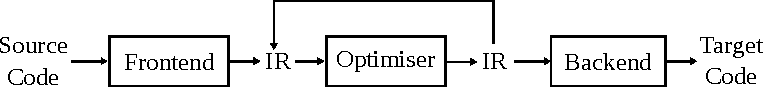
\includegraphics[width=\linewidth]{figs/3-phase-compiler.pdf}
    \caption{Overview of the three-phase compiler infrastructure.}
    \label{fig:3-phase-compiler}
\end{figure}


\chapter{Conclusions and Future Work}


%% ... etc ...

%%%%%%%%
%% Any appendices should go here. The appendix files should look just like the
%% chapter files.
\appendix
\chapter{Aliquam erat volutpat}


\textbf{If you need to add appendices, this is how you should do it:}

(If you're wondering what all this weirdness is, check out\\
http://www.subterrane.com/loremipsum.shtml)

Aliquam erat volutpat. Phasellus sed tortor at metus luctus venenatis.
Etiam vel dolor vel lectus elementum adipiscing. Donec sit amet dolor. In
hac habitasse platea dictumst. Nullam bibendum. Etiam eget mauris non velit
faucibus volutpat. Ut ultrices nonummy mi. Praesent convallis, tellus eget
posuere auctor, est est mollis risus, vitae fringilla orci nisl vel erat.
Morbi ultricies. Proin consequat. Praesent consequat nulla a mauris.
Vivamus tellus. 

\section{Proin consequat}

Sed blandit nunc id massa. Integer dictum euismod tellus. Sed metus nunc,
rhoncus ut, volutpat in, lacinia ac, dolor. Vestibulum quis augue
vel dui volutpat eleifend. Praesent vulputate mattis leo. Phasellus pretium
semper libero. Mauris a enim non pede convallis suscipit. Suspendisse nibh
diam, luctus in, cursus at, dignissim nec, pede. Aenean semper massa.
Pellentesque habitant morbi tristique senectus et netus et malesuada fames ac
turpis egestas. Nullam a pede ut ligula viverra vehicula. Sed augue mi,
rhoncus ut, ultrices sed, tincidunt eget, libero. Nam quis dolor. Nunc
fermentum hendrerit arcu. Integer non enim. Aenean blandit velit et felis. Cum
sociis natoque penatibus et magnis dis parturient montes, nascetur ridiculus
mus. Curabitur nonummy malesuada pede. Nunc et enim. Quisque dui. Pellentesque
in felis. 

Sed id mi. Pellentesque pede leo, auctor et, interdum eu, posuere semper,
nisl. Morbi commodo euismod wisi. Cras ornare mauris et erat. Duis neque
neque, pretium ut, bibendum nec, ultrices a, lacus. Nullam lobortis. Ut
luctus, diam non tempus pellentesque, dui justo consequat ligula, eu
consectetuer tortor diam vel dui. 

\begin{figure}
    \begin{center}
        A figure.
        \caption{Nunc lacinia}
    \end{center}
\end{figure}

Phasellus porttitor. In pede lacus, convallis semper, fermentum eu,
vehicula quis, dui. Ut sodales pede sed est. Cras lacinia. Nulla ac augue
in lectus sodales ultricies. Nam velit nunc, convallis ac, ullamcorper
semper, malesuada vel, eros. Nunc risus. Vestibulum ac erat. Sed id justo
id nibh viverra facilisis. Curabitur laoreet. Nunc sodales odio at mauris.
Vestibulum tincidunt sem eget pede. Nulla nec risus non wisi varius porta.
Morbi nibh. Donec lacus. Vestibulum ante ipsum primis in faucibus orci
luctus et ultrices posuere cubilia Curae; Vestibulum lectus. Suspendisse
sed dui. 

Nunc lacinia, sapien nec fermentum pretium, turpis elit egestas metus, a
interdum tellus justo semper neque. Integer quis purus semper metus
vestibulum pharetra. Maecenas commodo fermentum wisi. Pellentesque diam.
Proin sit amet orci. Praesent auctor. Sed tortor. Sed sodales aliquam diam.
Vivamus cursus leo nec velit. Sed non pede. Nulla tempor imperdiet est.
Curabitur ornare cursus ante. Sed varius lobortis quam. Quisque ac arcu id
wisi ultrices pellentesque. Pellentesque eleifend consequat ipsum. Fusce
vestibulum sagittis lectus. Fusce risus. Duis felis. Suspendisse justo.
Integer ut libero a purus egestas luctus. Mauris dictum augue a enim.
Vivamus sodales placerat ipsum. Nunc lacus. 

\begin{quote}
Curabitur dictum. Donec vestibulum diam nec lacus. Nulla convallis, eros
vitae varius volutpat, erat quam facilisis purus, in accumsan dolor felis
vitae nunc. 
\end{quote}

Aliquam erat volutpat. Phasellus sed tortor at metus luctus venenatis.
Etiam vel dolor vel lectus elementum adipiscing. Donec sit amet dolor. In
hac habitasse platea dictumst. Nullam bibendum. Etiam eget mauris non velit
faucibus volutpat. \footnote{Ut ultrices nonummy mi. Praesent convallis, tellus eget
posuere auctor, est est mollis risus, vitae fringilla orci nisl vel erat.
Morbi ultricies.} Proin consequat. Praesent consequat nulla a mauris.
Vivamus tellus. 

Phasellus porttitor. In pede lacus, convallis semper, fermentum eu,
vehicula quis, dui. Ut sodales pede sed est. Cras lacinia. Nulla ac augue
in lectus sodales ultricies. Nam velit nunc, convallis ac, ullamcorper
semper, malesuada vel, eros. Nunc risus. Vestibulum ac erat. Sed id justo
id nibh viverra facilisis. Curabitur laoreet. Nunc sodales odio at mauris.
Vestibulum tincidunt sem eget pede. Nulla nec risus non wisi varius porta.
Morbi nibh. Donec lacus. Vestibulum ante ipsum primis in faucibus orci
luctus et ultrices posuere cubilia Curae; Vestibulum lectus. Suspendisse
sed dui. 

Sed id mi. Pellentesque pede leo, auctor et, interdum eu, posuere semper,
nisl. Morbi commodo euismod wisi. Cras ornare mauris et erat. Duis neque
neque, pretium ut, bibendum nec, ultrices a, lacus. Nullam lobortis. Ut
luctus, diam non tempus pellentesque, dui justo consequat ligula, eu
consectetuer tortor diam vel dui. 


%% ... etc...

%% Choose your favourite bibliography style here.
\bibliographystyle{apalike}

%% If you want the bibliography single-spaced (which is allowed), uncomment
%% the next line.
% \singlespace

%% Specify the bibliography file. Default is thesis.bib.
\bibliography{bibliography}

%% ... that's all, folks!
\end{document}
